% vim: spell spelllang=en:
%! TEX root = **/00-main.tex

% Hierarchical Clustering on original data:

\section{Hierarchical Clustering}%
\label{sec:hierarchical_clustering}

\subsection{Description of data}%
\label{sub:description_data}
% TODO:

% Precise description of the data used (which variables have not been included
% in the analysis, if any, whenever you are using a CURE strategy, provide
% details about eventual sampling performed on data, etc)

We decided to investigate two different hierarchical clustering methods to
identify which one worked best with our data set: Ward's hierarchical method and 
Hierarchical Clustering on Principal Components (HCPC). The script for both methods
can be found in \cref{sub:clustering.r}. Ward uses
the whole preprocessed data set while HCPC uses the PCA outcome. None of the
methods required any kind of sampling.

\subsection{Methods, metrics and criteria}

% Clustering method used, metrics and aggregation criteria used (Ward’s method
% is recommended embedded or not in a CURE strategy whenever scaling to big data
% is required, for messy data Gower dissimilarity coefficient to the square is
% recommended )

As mentioned in \cref{sub:description_data}, we explored two different clustering methods.
Ward chooses which two clusters to merge based on the pair of clusters that leads to the
minimum increase in the sum of squared Euclidean distances for the merged cluster. 
On the other hand, HCPC applies the same Ward criterion but on the principal components 
not to the whole data set.


\subsection{Dendogram and number of clusters}%
\label{sub:dendogram}

% Resulting Dendrogram (of the total dataset or the sample). USE A SINGLE PAGE
% for it

\begin{figure}[H]
    \centering
    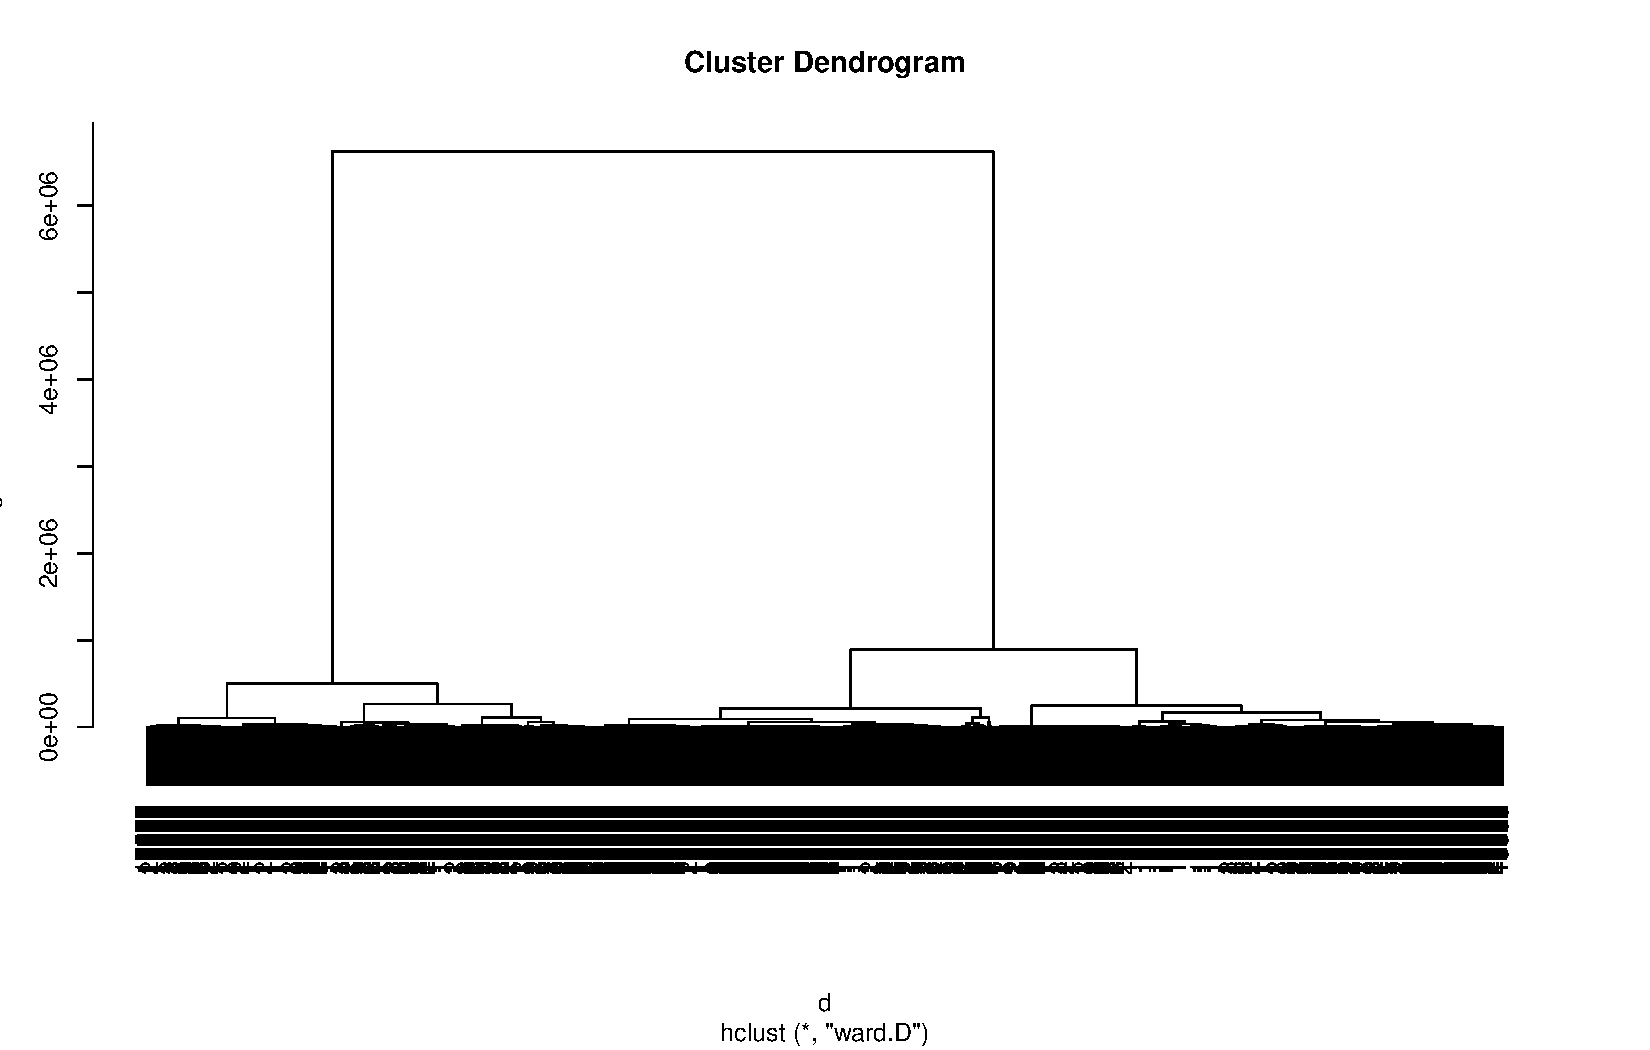
\includegraphics[width=0.8\linewidth]{cluster-dendo-h1}
    \caption{Cluster Dendogram}%
    \label{fig:dendogram-h2}
\end{figure}

This is the dendogram for the Ward hierarchical clustering, which we decided to split into 3 clusters
as they were evenly sized, see \cref{sub:description_of_clusters}. While the cluster 
partitions are uniform in size and at first it may look promising, we found out by examining 
the clusters in detail that HCPC provided better results. For that reason we chose to study the
cluster profiling for HCPC.

\begin{landscape}

\begin{figure}[H]
    \centering
    %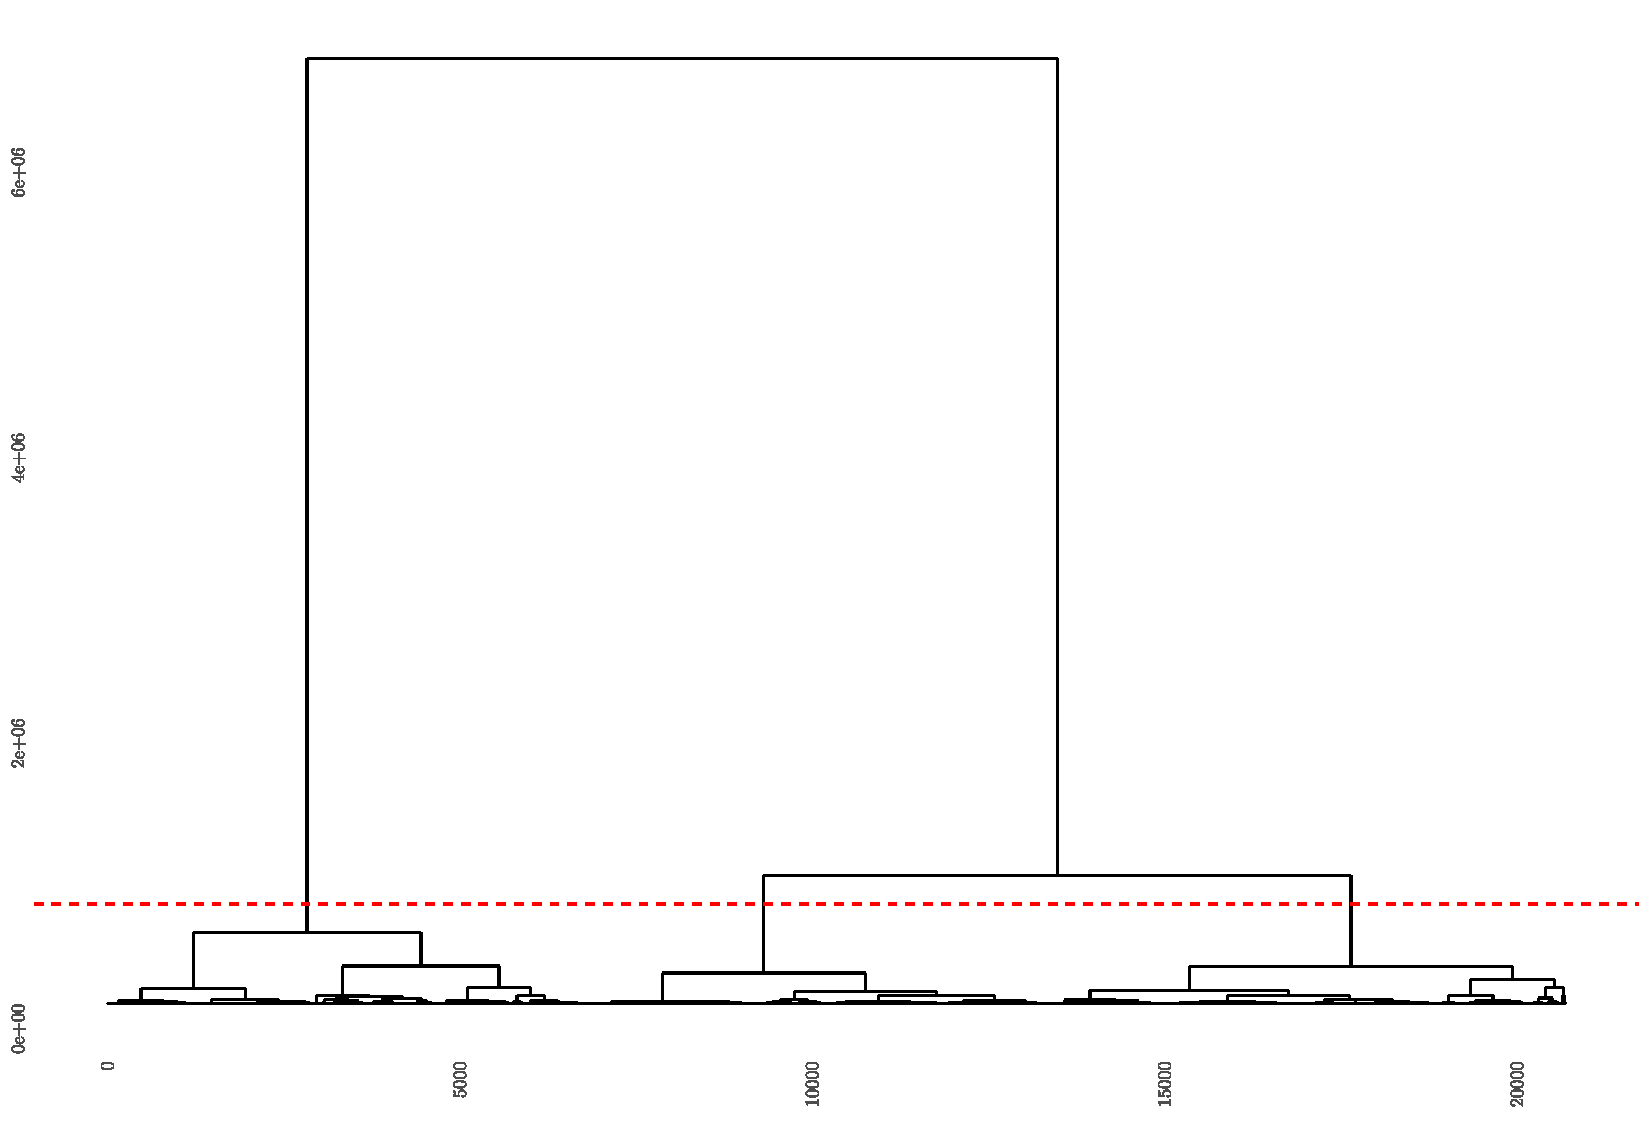
\includegraphics[width=0.8\linewidth]{dendo}
    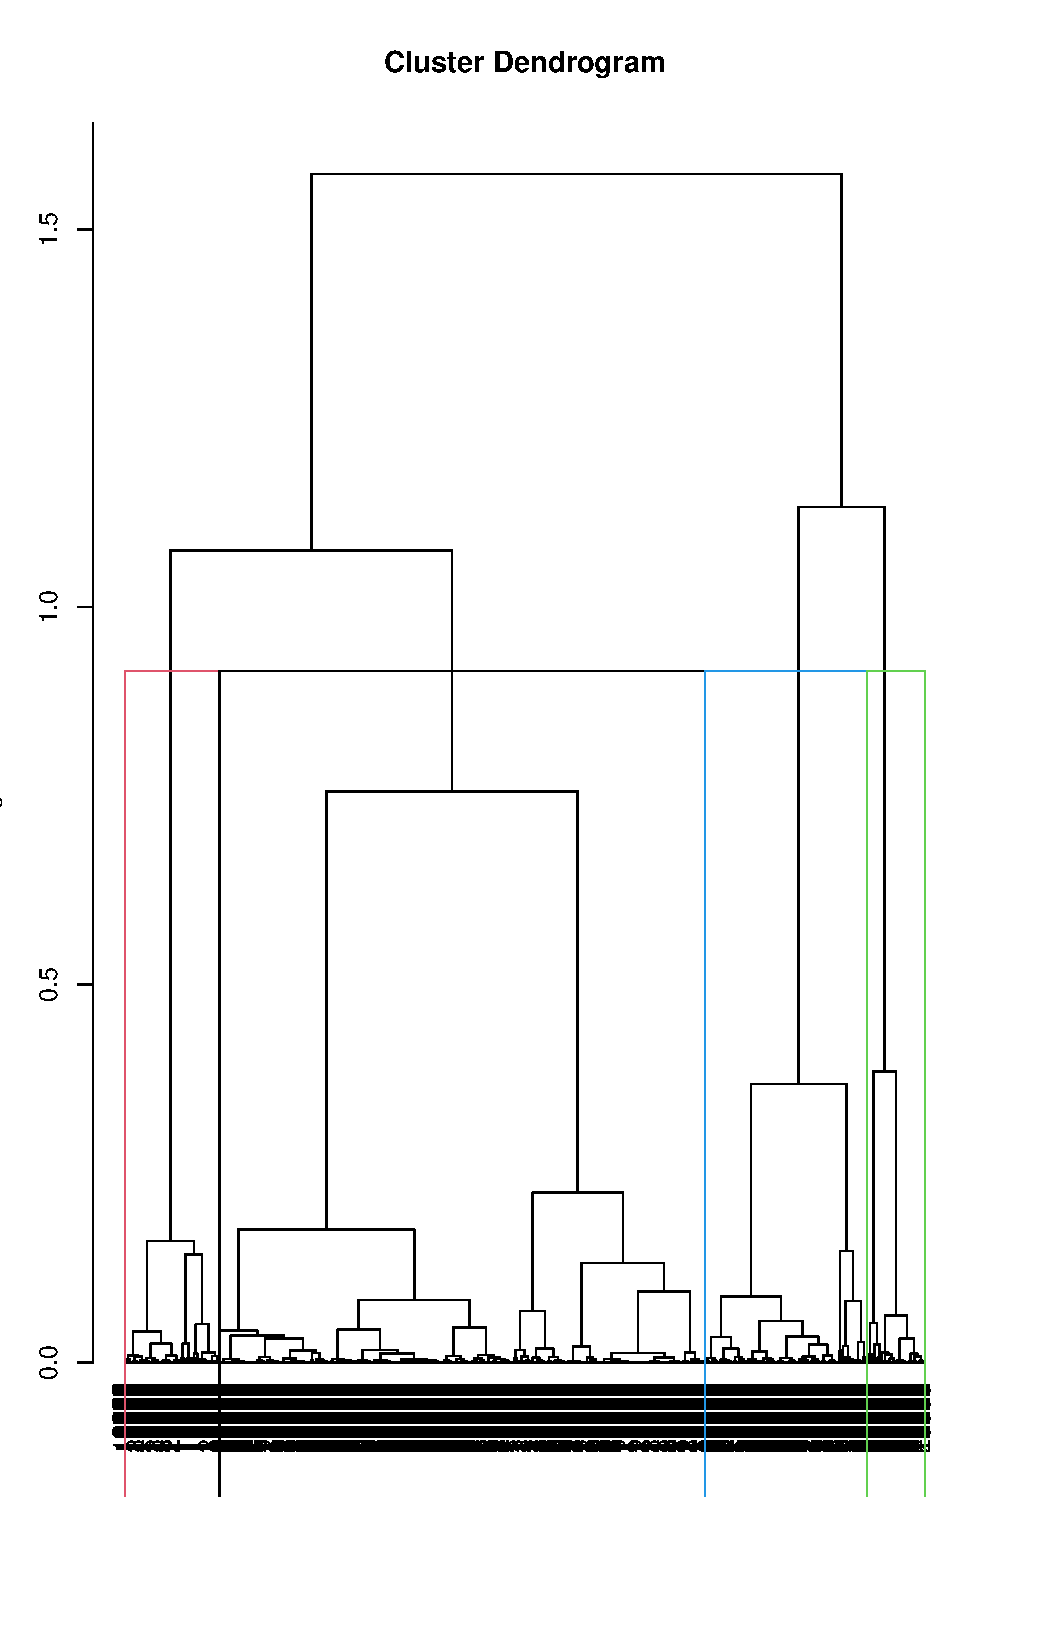
\includegraphics[width=0.8\linewidth]{cluster-dendo-h3}
    \caption{Cluster Dendogram}%
    \label{fig:dendogram-final}
\end{figure}

\end{landscape}

The dendogram in \cref{fig:dendogram-final} corresponds to HCPC. When calling FactoMineR's \texttt{HCPC}
function to calculate the clusters, we set the argument \texttt{nb.clust} to -1 in order to obtain the
suggested cut, which in this case is at level 4.

% Discuss about how to get the final number of clusters

\subsection{Description of clusters}%
\label{sub:description_of_clusters}

As a result of the cut levels mentioned before, we obtained the following cluster sizes.
For Ward's method the clusters are equitably sized, as we can appreciate in
\cref{tab:cluster_size_ward}. On \cref{tab:cluster_size_hcpc}, we can observe that
the cluster sizes aren't as homogeneous, with cluster 1 absorbing more than half
of all data records at 12,733. Then we have cluster 4 with a size of 4,414 and cluster 2
taking 2,378. Finally, cluster 3 only contains 810 records.

\begin{table}[h!]
\vspace{5pt}
\caption{Cluster size table}%
\label{tab:cluster_size}
\centering
\begin{subtable}[t]{.3\textwidth}
    \centering
    \caption{Ward cluster size}%
    \label{tab:cluster_size_ward}
    
\begin{tabular}[t]{cr}
\toprule
Cluster & Freq\\
\midrule
1 & 6783\\
2 & 6101\\
3 & 7811\\
\bottomrule
\end{tabular}
\end{subtable}
\begin{subtable}[t]{.3\textwidth}
    \centering
    \caption{HCPC cluster size}%
    \label{tab:cluster_size_hcpc}
    
\begin{tabular}[t]{lr}
\toprule
c3 & Freq\\
\midrule
1 & 12733\\
2 & 2738\\
3 & 810\\
4 & 4414\\
\bottomrule
\end{tabular}
\end{subtable}
\end{table}

\begin{figure}[H]
\centering
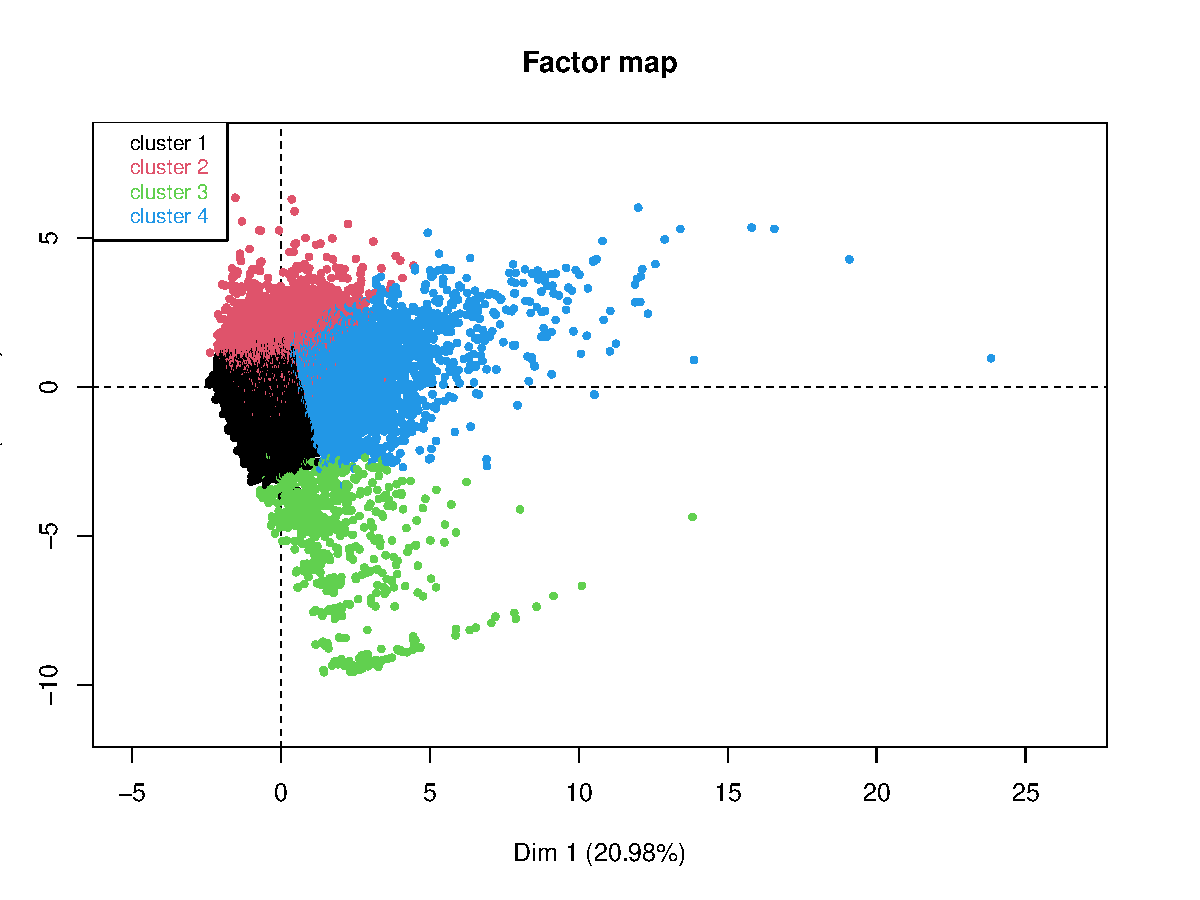
\includegraphics[width=0.7\linewidth]{factor_map}
\caption{Clusters on PCA}%
\label{fig:clusters-pca}
\end{figure}

In \cref{fig:clusters-pca} we can view the HCPC cluster divisions on a PCA factor map.

% Table with a description of the clusters size
